\documentclass[letterpaper, 12pt]{article}
\usepackage[utf8]{inputenc}
\usepackage[english, spanish]{babel}
\usepackage{fullpage} % changes the margin
\usepackage{graphicx}
\usepackage{enumitem}
\usepackage{chngcntr}
\usepackage{multirow}
\usepackage{parskip}
\usepackage{url}
\usepackage{booktabs} 
\counterwithin{figure}{section}
\renewcommand{\thesection}{\arabic{section}}
\renewcommand{\thesubsection}{\thesection.\arabic{subsection}}
\renewcommand{\baselinestretch}{1.5}
\usepackage{float}
\usepackage{apacite}
\usepackage{multicol}
\bibliographystyle{apacite}
\setlength\belowcaptionskip{10pt}
\linespread{1.5}

\begin{document}

\begin{titlepage}
	\centering
	
\includegraphics[width=0.3\textwidth]{Images/logo_utb.png}\par\vspace{1cm}
	{\scshape\LARGE Universidad Tecnológica de Bolívar \par}
	\vspace{1cm}

	{\scshape\Large FÍSICA ELÉCTRICA \par}
	\vspace{.2cm}

	% chktex-file 8
	{\scshape\Large H1 - C \par}
	\vspace{1cm}
	% chktex-file 8
	\slshape {\Large \bfseries{}Informe de Laboratorio No.  \\}
	\vspace{1cm}

	\slshape {\itshape{} Mauro González, T00067622 \\}
	\slshape {\itshape{} German De Armas Castaño, T00068765 \\}
	\slshape {\itshape{} Angel Vega Rodriguez, T00068186 \\}
	\slshape {\itshape{} Juan Jose Osorio Ariza, T00067316 \\}
	\slshape {\itshape{} Juan Eduardo barón, T00065901 \\}
	\vfill
	Revisado Por \\
	Gabriel Hoyos Gomez Casseres\\
	{\large \today\par}
\end{titlepage}

% ----------------------------------------------------------------------|>
\section{Introducción}

% \newpage

% ----------------------------------------------------------------------|>
\section{Objetivos}

\subsection{Objetivos General}

% \newpage

% ----------------------------------------------------------------------|>
\section{Marco Teórico}

% ---------------------------------------------------|>
\subsection*{Ley de Ohm}

La Ley de Ohm establece que la corriente eléctrica que fluye a través de un
circuito es proporcional a la diferencia de potencial eléctrico entre los
extremos del mismo, y es inversamente proporcional a la resistencia del
circuito.~\cite{LeyDeOhm}

% ---------------------------------------------------|>
\subsection*{Material tipo Ohm}

Los materiales óhmicos tienen una relación lineal de corriente-diferencia de
potencial en un largo intervalo de diferencias de potencial aplicadas.
La pendiente de la curva I v/s $\triangle$V en la región lineal produce un
valor para 1/R.~\cite{MaterialesOhmicos}

% ---------------------------------------------------|>
\subsection*{Deducción a partir de la ley de Ohm}

La resistencia de un conductor cilíndrico está determinada por su longitud $l$,
la sección transversal $a$ y la resistividad del material a una temperatura dada.
La resistencia es directamente proporcional a la longitud $l$ y a la
resistividad $\rho$, pero inversamente proporcional a su sección transversal.

$R = p \cdot \frac{l}{a}$

% ---------------------------------------------------|>
\subsection*{Factores de los cuales depende la resistencia y resistividad}

La resistividad de un material óhmico es una propiedad característica que
depende de su composición y temperatura. Los materiales con resistividad
cero son considerados conductores ideales, mientras que aquellos con
resistividad infinita son considerados aislantes ideales. En otras
palabras, la resistividad de un material es un factor clave en la
determinación de su capacidad para conducir electricidad.

% ---------------------------------------------------|>
\subsection*{Temperatura, resistencia y resistividad}

La resistividad $\rho$ de un material depende de la estructura molecular y
atómica, y es dependiente de la temperatura. Para la mayoría de los conductores,
la resistividad aumenta con el aumento de temperatura.~\cite{KhanAcademy}

% ---------------------------------------------------|>
\subsection*{Gráfica de Voltaje vs Corriente}

\begin{figure}[H]
	\begin{center}
		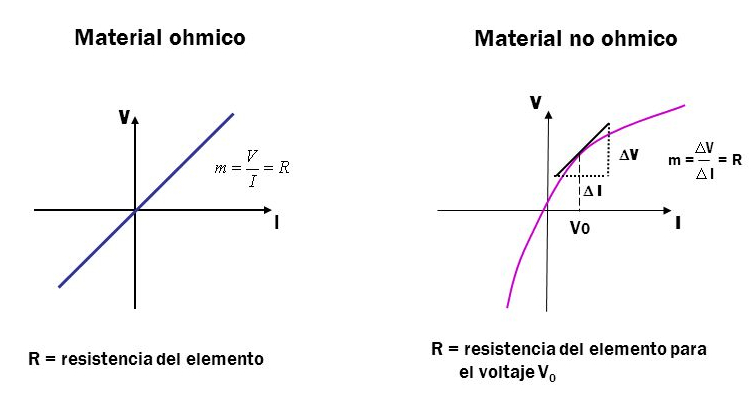
\includegraphics[scale = 0.5]{./Images/VoltajeVsResistencia.jpg}
	\end{center}
\end{figure}


% ----------------------------------------------------------------------|>
\section{Montaje Experimental}

% ----------------------------------------------------------------------|>
\section{Datos Experimentales}

\begin{table}[H]
	\centering
	\caption{Tabla de valores para resistencia eléctrica}
	% chktex-file 24
	\label{tabla-resistencia 1ra Medicion}
	\begin{tabular}{cccccccc}
		\toprule
		                          & 1      & 2                                    & 3                     & 4        & 5      & 6     & 7     \\
		\midrule
		R ($\Omega$)              & 0.6    & 1.6                                  & 1.8                   & 2        & 2.4    & 2.8   & 3.3   \\
		L/A ($m^{-1}$)            & 0.07   & 0.14                                 & 0.21                  & 0.28     & 0.35   & 0.42  & 0.49  \\
		$\rho$ ($\Omega \cdot m$) & 0.042  & 0.224                                & 0.378                 & 0.56     & 0.84   & 1.176 & 1.617 \\
		Promedio: $\rho$          & 0.5367 & \multicolumn{2}{c}{Área Transversal} & $4.71 \times 10^{-4}$ & Material & Blanck                 \\
		\bottomrule
	\end{tabular}
\end{table}

\begin{table}[H]
	\centering
	\caption{Tabla de valores para resistencia eléctrica}
	% chktex-file 24
	\label{tabla-resistencia 2da Medicion}
	\begin{tabular}{cccccccc}
		\toprule
		                          & 1      & 2                                    & 3                     & 4        & 5      & 6     & 7    \\
		\midrule
		R ($\Omega$)              & 1.5    & 2                                    & 2.8                   & 3.7      & 4.4    & 5.2   & 6    \\
		L/A ($m^{-1}$)            & 0.07   & 0.14                                 & 0.21                  & 0.28     & 0.35   & 0.42  & 0.49 \\
		$\rho$ ($\Omega \cdot m$) & 0.105  & 0.28                                 & 0.588                 & 1.036    & 1.54   & 2.184 & 2.94 \\
		Promedio: $\rho$          & 0.9555 & \multicolumn{2}{c}{Área Transversal} & $6.28 \times 10^{-4}$ & Material & Blanck                \\
		\bottomrule
	\end{tabular}
\end{table}

% \begin{table}[H]
% 	\begin{tabular}{ccc}
% 		\label{tabla-resistor 1ra Medicion}
% 		\toprule
% 		Voltaje $(V)$ & Corriente I $(mA)$ & Escala  \\
% 		\midrule
% 		0.566         & 1                  & $10mA$  \\
% 		1.016         & 2                  &         \\
% 		1.555         & 3                  &         \\
% 		2.032         & 4                  &         \\
% 		2.57          & 5                  &         \\
% 		3.058         & 6                  &         \\
% 		3.56          & 7                  &         \\
% 		4.3           & 8                  &         \\ % chktex-file 44
% 		4.57          & 9                  &         \\
% 		\midrule
% 		4.80          & 10                 & $100mA$ \\
% 		5.09          & 11                 &         \\
% 		5.3           & 12                 &         \\
% 		6.39          & 13                 &         \\
% 		6.80          & 14                 &         \\
% 		\bottomrule
% 	\end{tabular}
% \end{table}

% \begin{table}[H]
% 	\begin{tabular}{ccc}
% 		\label{tabla-resistor 2da Medicion}
% 		\toprule
% 		Voltaje $(V)$ & Corriente I $(mA)$ & Escala \\
% 		\midrule
% 		0.5           & 0.4                & $3mA$  \\
% 		1.0           & 0.5                &        \\
% 		1.5           & 0.6                &        \\
% 		2.0           & 0.7                &        \\
% 		2.5           & 0.8                &        \\
% 		3.0           & 0.85               &        \\
% 		3.5           & 0.9                &        \\
% 		4.0           & 1                  &        \\
% 		4.5           & 1.05               &        \\
% 		5.0           & 1.1                &        \\
% 		5.5           & 1.15               &        \\
% 		6.0           & 1.2                &        \\
% 		6.5           & 1.25               &        \\
% 		7.0           & 1.3                &        \\
% 		7.5           & 1.35               &        \\
% 		8.0           & 1.4                &        \\
% 		8.5           & 1.45               &        \\
% 		9.0           & 1.5                &        \\
% 		9.5           & 1.55               &        \\
% 		10            & 1.6                &        \\
% 		\bottomrule
% 	\end{tabular}
% \end{table}

\newpage

\begin{multicols}{2}

	\begin{figure}[H]
		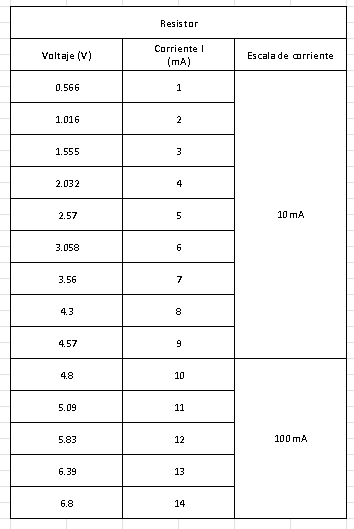
\includegraphics[scale = .6]{./Images/Table1.png}
	\end{figure}

	\begin{figure}[H]
		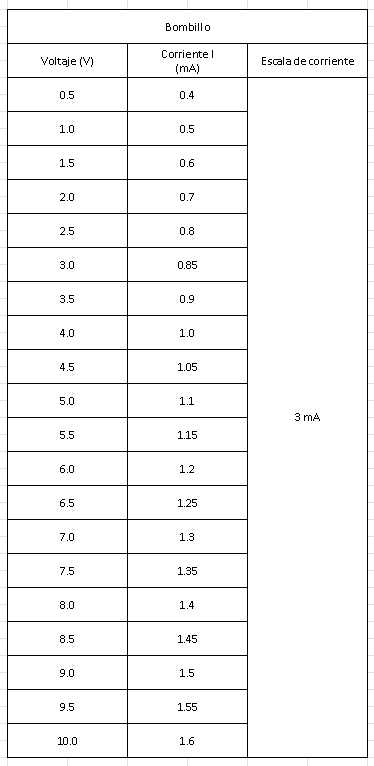
\includegraphics[scale = .64]{./Images/Table2.png}
	\end{figure}

\end{multicols}

% ----------------------------------------------------------------------|>
\section{Análisis de datos}

% --------------------------------------------|>
\subsection*{Calcule el área transversal A (en m2)
	de uno de los alambres utilizados}

$A = \pi \cdot R$

Usando esta formula, hallamos el area transversal
$A = \pi \cdot (\frac{0.3}{2000}) => 6.28 \times 10^{-4}$

% --------------------------------------------|>
\subsection*{Compare el valor de resistividad encontrado de los diferentes materiales
	registrados en la tabla 4.}

% --------------------------------------------|>
\subsection*{Compare el valor de resistividad encontrado de los diferentes materiales
	registrados en la tabla 4.}

% --------------------------------------------|>
\subsection*{¿A qué se debe la diferencia entre el valor de resistividad encontrado y registrado
	en las tablas?}
	
% --------------------------------------------|>
\subsection*{¿Depende la resistividad de la longitud del alambre?}

% --------------------------------------------|>
\subsection*{¿Depende la resistividad de la longitud del alambre?}

% --------------------------------------------|>
\subsection*{¿Depende la resistividad del área transversal del alambre?}

% --------------------------------------------|>
\subsection*{¿Depende la resistividad del área transversal del alambre?}



























% ----------------------------------------------------------------------|>
\section{Conclusiones}

\newpage

\bibliography{./Bibliography/bibliography.bib}

\end{document}